\section{Приборы, используемые в работе}
\addcontentsline{toc}{section}{Приборы, используемые в работе}	% Добавляем его в оглавление

\begin{center}
  \begin{longtable}{| m{0.5cm} | m{3cm} | m{1.5cm} | m{2cm} | m{8cm}l |}
  
  \hline
  \centering № & \centering Наименование &\centering Тип &\centering Заводской номер &\centering Основные технические характеристики & \\
  \hline
  \centering 1 &\centering Генератор сигналов низкочастотный &\centering Г4-117 &\centering &\centering
Диапазон генерируемых частот:\par 20 Гц $ ... $ 10 МГц\par
Относительная погрешность установки: $ \pm (0,02f + 1)$ Гц;\par
на участке 100 $ ... $ 200 Гц: \par $ \pm (0,02f+4) $ Гц.\par
Основная погрешность установки выходного напряжения по шкале стрелочного индикатора не превышает $ 10 \% $ от номинального конечного значения соответствующей шкалы. &  \\

	\hline
	\centering 2 &
	\centering Осциллограф универсальный двухканальный &
	\centering C1-117 &
	&
	\centering Предел измерений: 10 МГц \par Погрешность коэффициента: $ \pm4 \% $ &
	\\

  \hline
  \centering 3 &
  \centering Генератор импульсов &
  \centering В5-54 & 
  &
  \centering Предел измерений: 50 В \par Погрешность установки: \par не более $ \pm(0,1 U_{m}$+К $ 1,0) $ В, \par где К - коэффициент ступенчатого ослабления &
	\\
  
  \hline    
  
  \end{longtable}
\end{center}

\begin{figure}[htbp]
  \center{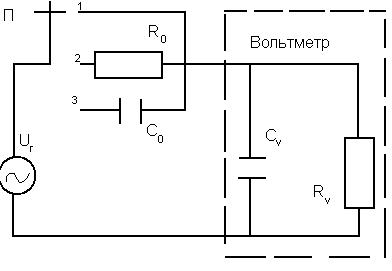
\includegraphics[width=0.8\linewidth]{scheme1}}
  \caption{Структурная схема изучаемого осциллографа}
\end{figure}

\begin{figure}[!h]
  \center{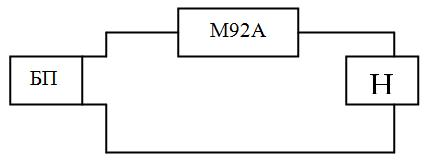
\includegraphics[width=0.8\linewidth]{scheme2}}
  \caption{Схема лабораторного макета}
\end{figure}

\clearpage
